Portugal is a country in Europe with a resident population of around 10.2 million inhabitants.  \\
According to the Nacional Statistics Institute, INE (Instituto Nacional de Estatística),  \cite{pubINE} in "Demographic Statistics - 2019":
\begin{itemize}
    \item Concerning to \textbf{sex},
    \begin{itemize}
        \item \textbf{47,2\textdiscount} of the population is \textbf{male};
        \item \textbf{52,8 \textdiscount} of the population is \textbf{female}.
\begin{figure}[h!]
\caption{Portugal: Gender Distribution}
\centering
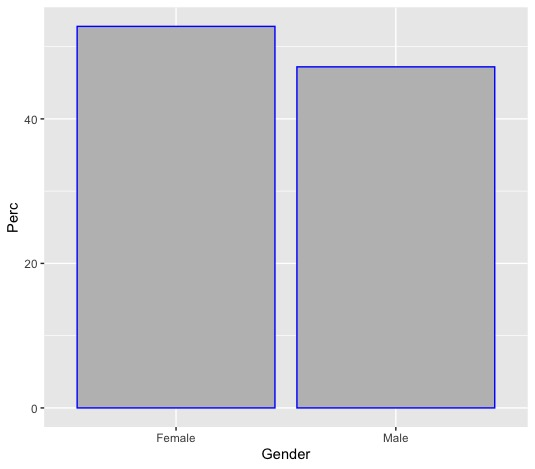
\includegraphics[width=0.6\textwidth]{Sex.jpeg}
\end{figure}
    \end{itemize}  
    \item In terms of \textbf{age},
    \begin{itemize}
        \item \textbf{13,6\textdiscount} of \textbf{young people} (0-14 y/o);
        \item \textbf{64.3\textdiscount} of people of \textbf{active people} (15-64 y/o);
        \item \textbf{22.1\textdiscount} of \textbf{elderly people} (65+ y/o). 
\begin{figure}[h!]
\caption{Portugal: Age Distribution}
\centering
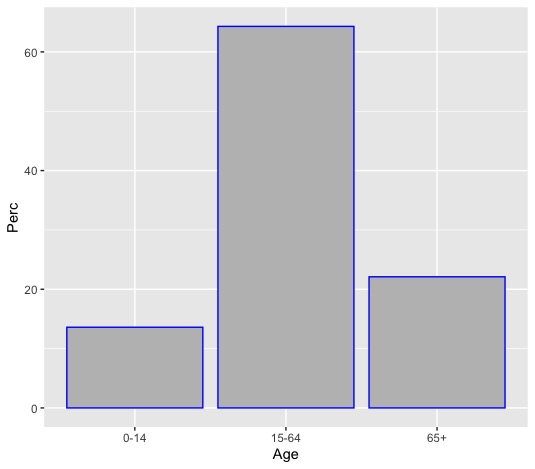
\includegraphics[width=0.8\textwidth]{Age.jpeg}
\end{figure}
    \end{itemize}
\end{itemize}
